\chapter*{Introduction}                         % Заголовок
\addcontentsline{toc}{chapter}{Introduction}    % Добавляем его в оглавление

\newcommand{\actuality}{}
\newcommand{\challanges}{}
\newcommand{\progress}{}
\newcommand{\aim}{{\textbf\aimTXT}}
\newcommand{\tasks}{\textbf{\tasksTXT}}
\newcommand{\novelty}{\textbf{\noveltyTXT}}
\newcommand{\influence}{\textbf{\influenceTXT}}
\newcommand{\methods}{\textbf{\methodsTXT}}
\newcommand{\defpositions}{\textbf{\defpositionsTXT}}
\newcommand{\reliability}{\textbf{\reliabilityTXT}}
\newcommand{\probation}{\textbf{\probationTXT}}
\newcommand{\contribution}{\textbf{\contributionTXT}}
\newcommand{\publications}{\textbf{\publicationsTXT}}


{\actuality} 
The Fourth Industrial Revolution (Industry 4.0) is characterized by the integration of digital technologies into manufacturing and production systems, significantly transforming energy management and consumption. This transition, shown in Figure~\cref{fig:industry4}, is particularly evident in the increased reliance on electrical energy as a key production resource, impacting both industrial and household consumers who are increasingly sensitive to the quality and stability of electrical energy supply \autocite{He_2022}.

\begin{figure}[ht]
    \centerfloat{
        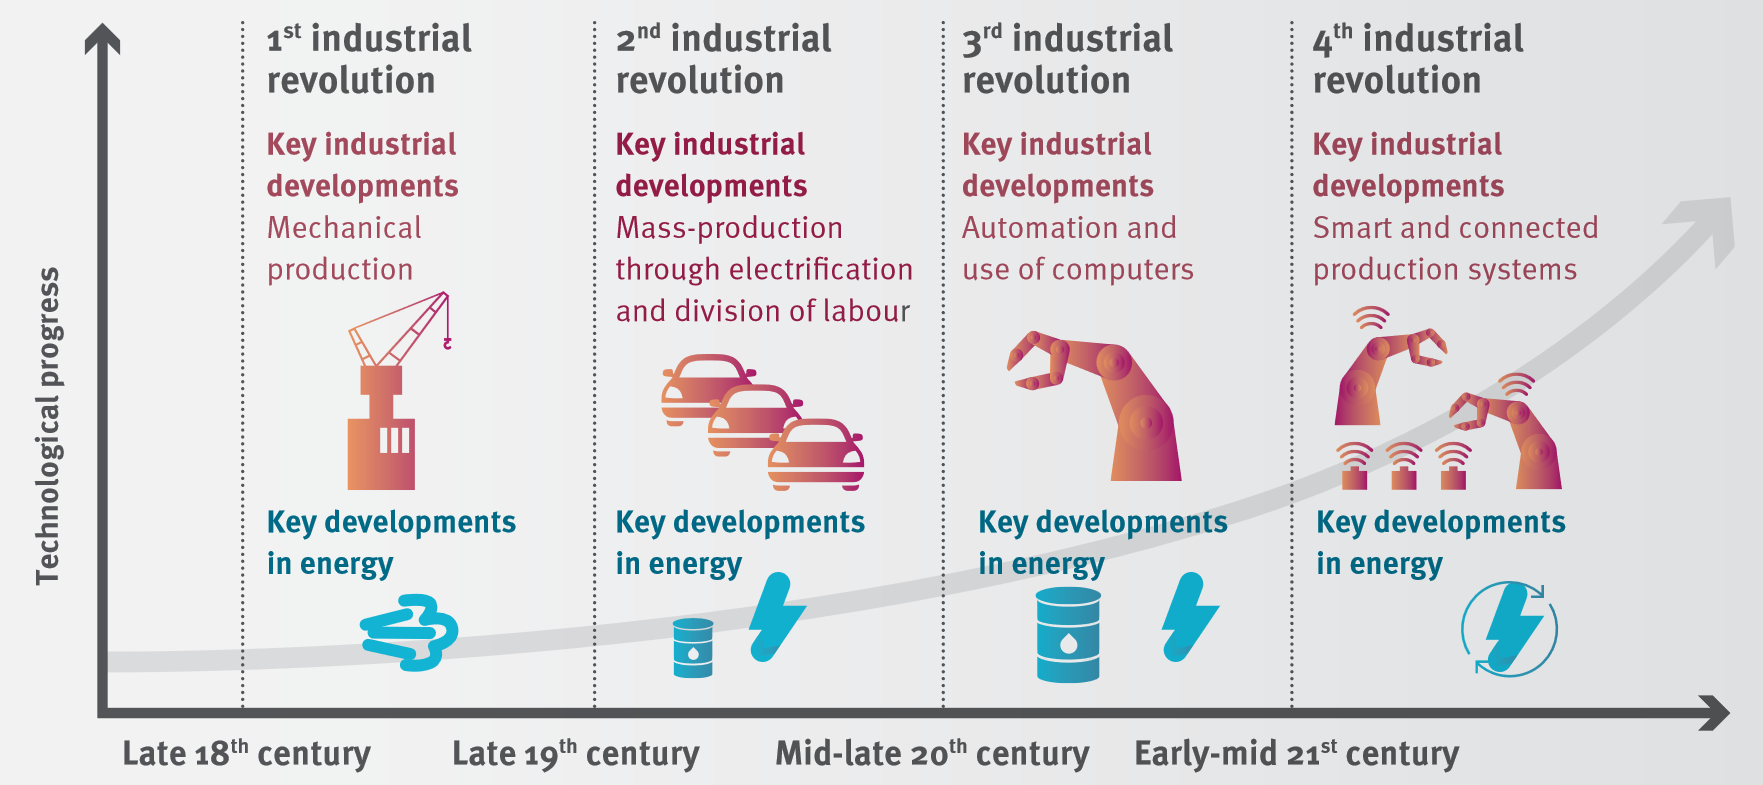
\includegraphics[scale=0.33]{industry4}
    }
    \caption{Industrial revolutions and key developments in energy change \cite{UNIDO2017}.}\label{fig:industry4}
\end{figure}

A new era of technological and social transformation is reshaping consumer expectations for energy systems, with the following required features \autocite{kholkin2025energy}:
\begin{itemize}
    \item  \textbf{Quality}: capability of power supply systems to meet the growing digital demand segment by delivering electricity with high reliability and performance standards, supported by energy storage systems (ESS), power electronics and digital control technologies.
    
    \item  \textbf{Autonomy}: energy resilience of settlements, individual consumers, mobile devices, and transport systems, enabled by local generation, storage, high-density energy conversion and smart grids, reducing reliance on centralized power and fuel supply.
    
    \item  \textbf{Intelligence}: digital modeling, scalable architectures, and digital markets enable dynamic energy exchange, automated control of complex infrastructure, and customized services to meet evolving demand.
\end{itemize}

\nomenclature{\(ESS\)}{Energy Storage Systems}


% \section{Challenges in microgrid operation and control}
\textbf{Challenges in microgrid operation and control.}
To satisfy consumer expectations, the global energy landscape is undergoing a significant transformation, driven by the increasing adoption of distributed energy systems that integrate various energy sources, including renewable generation (solar, wind), ESS, electric vehicles (EV) and controllable loads. Furthermore, the integration of renewable energy resources (RES) and distributed energy resources (DER) into the grid is typically achieved through inverter-based resources (IBR). The significant benefits of such systems in terms of energy security, sustainability, and economic efficiency, lead power grids to evolve into power electronics dominated grids (PEDG) \autocite{mag_ipakchi_2009}, as shown in Figure~\cref{fig:bulk2pedg}. This transition results in an amplified complexity and significance for device and system-level control schemes to maintain resiliency, reliability and operational stability \autocite{mag_khan_2020}. 

\nomenclature{\(EV\)}{Electric Vehicles}
\nomenclature{\(PEDG\)}{Power Electronics Dominated Grid}
\nomenclature{\(DER\)}{Distributed Energy Resources}
\nomenclature{\(IBR\)}{Inverter-Based Resources}
\nomenclature{\(RES\)}{Renewable Energy Resources}

\begin{figure}[ht]
    \centerfloat{
        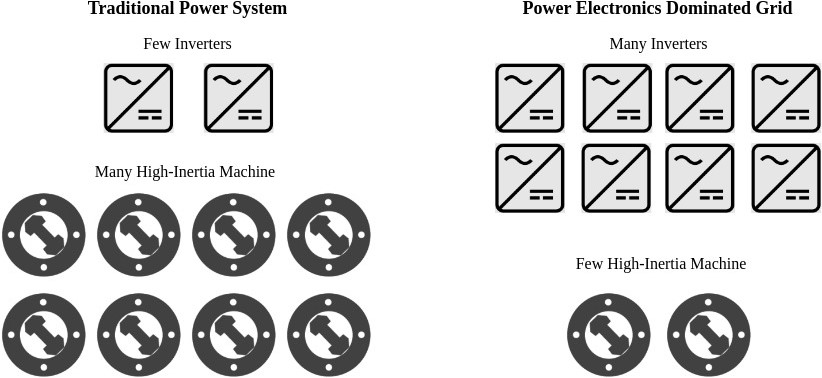
\includegraphics[scale=0.7]{bulk2pedg}
    }
    \caption{Transformation of energy paradigm.}\label{fig:bulk2pedg}
\end{figure}

As can be seen in Figure~\cref{fig:pedg_time}, the characteristic time scale of power electronics devices ranges from microseconds to milliseconds, introducing rapid control loops for voltage, current and phase-locked loops (PLL) of the network inverters. In other words, PEDG has low mechanical inertia and rapid and multi-timescale dynamics \autocite{7182342}, while also considering the inherent stochastic nature of its energy resources.

\nomenclature{\(PLL\)}{Phase-Locked Loop}

The reduced presence of synchronous machines in PEDG compared to static power electronics-based generators has a substantial impact on system inertia. PEDG exhibit significantly lower inertia than bulk interconnected power systems. This low inertia, coupled with the low short-circuit capacity of the network, exacerbates the challenge of maintaining stability. Even minor deviations in PEDG architecture due to intentional load or generator disconnections can lead to drastic fluctuations in voltage and frequency. The mixture of synchronous machines and inverter-based generation units introduces a combination of large and small time constants in PEDG, potentially causing unintended shutdowns of inverter-based generation units during system perturbations.

\begin{figure}[ht]
    \centerfloat{
        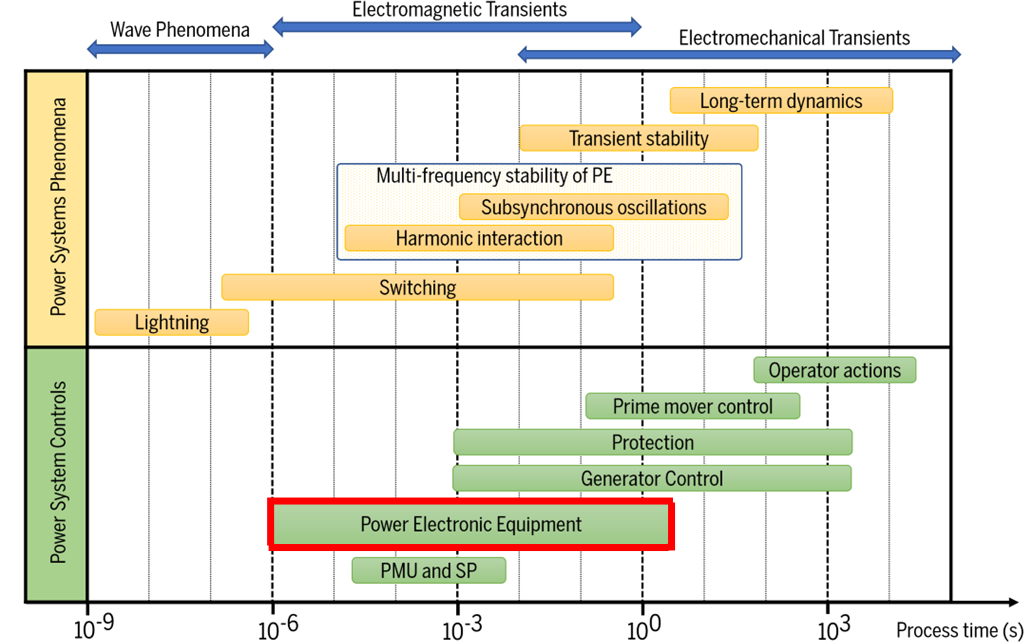
\includegraphics[scale=0.55]{pedg_time}
    }
    \caption{Characteristic operational time of PEDG \autocite{misc_karawita_2024}.}\label{fig:pedg_time}
\end{figure}

The intermittent nature of renewable energy sources in PEDG poses significant challenges for balancing demand and supply \autocite{7790991,7442160}. Moreover, the bidirectional power flow inherent in PEDG necessitates complex control and protection coordination among prosumers. It affects short-circuit current calculations and protection system design \autocite{4112346}, where engineers must consider the reserve for increased fault current magnitudes and the need to adjust protection settings to account for changed system characteristics. 

Furthermore, compared to the traditional bulk power system, PEDG exhibits unique characteristics due to the proximity of generation and load, resulting in shorter feeders and a lower inductance-resistance ratio (X/R) of grid impedance. In turn, it makes voltage control more challenging, requiring a careful management of reactive power \autocite{7749289}. 

Another key aspect, related with X/R ratio, is the equivalent impedance of the grid. The grid impedance plays a crucial role in determining the performance of IBRs. The performance of inverters is influenced not only by the inherent impedance of the power lines but also by the equivalent grid impedance at the Point of Common Coupling (PCC) as determined by the Thevenin equivalent circuit in Figure~\cref{fig:thevenin}. This impedance can be altered by the connection of parallel-connected inverters, further impacting the operation of other grid-connected devices \autocite{Jayasinghe2021}.

\nomenclature{\(PCC\)}{Point of Common Coupling}

\begin{figure}[ht]
    \centerfloat{
        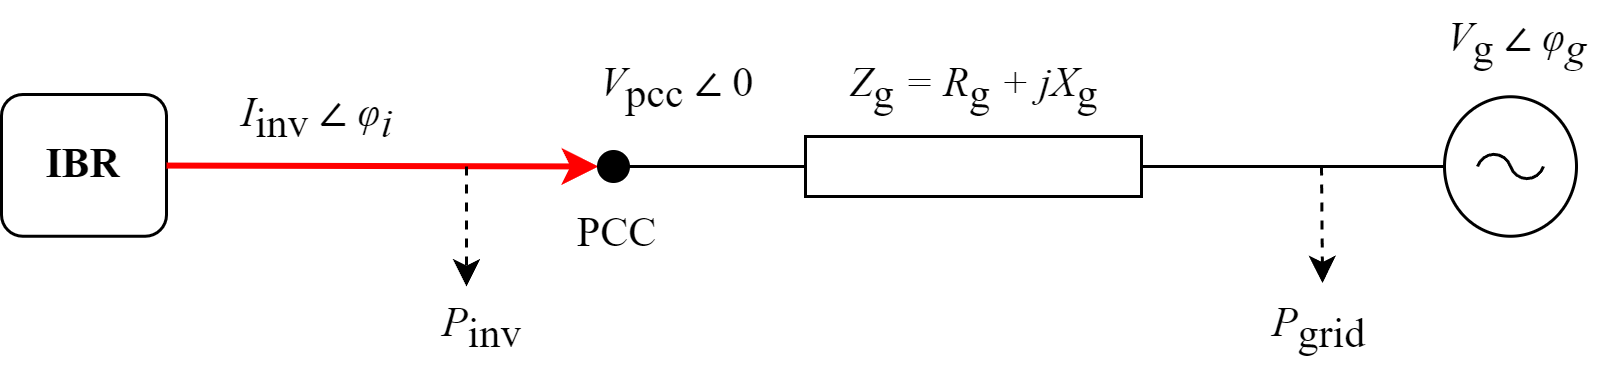
\includegraphics[scale=1.1]{thevenin}
    }
    \caption{Thevenin equivalent circuit of the grid-connected generation system.}\label{fig:thevenin}
\end{figure}

As the interconnection between multi-parallel inverters is established through the grid impedance, as shown in Figure~\cref{fig:multi_parallel}, the connection or disconnection of an inverter induces changes in the impedance seen by other inverters. This can threaten the ability of the power system to return to its normal conditions after disturbance, which is the stability of these inverters \autocite{10615092}, what is particularly relevant for low-voltage distribution systems with a lot of DERs. The fast dynamics of IBRs along with the inverter system moving to stable or unstable region can be resulted in current oscillations, as shown in Figure~\cref{fig:stability_regions}.

\begin{figure}[ht]
    \centerfloat{
        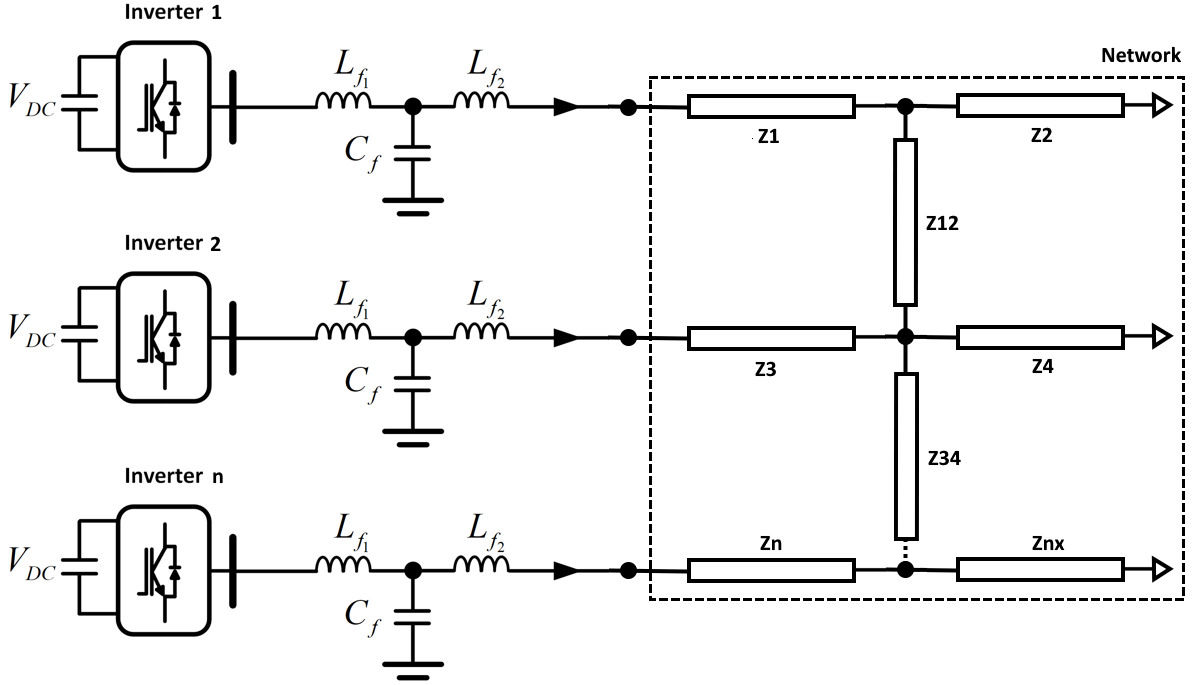
\includegraphics[scale=2]{multi_parallel}
    }
    \caption{Typical configuration of multiple paralleled inverters within a microgrid.}\label{fig:multi_parallel}
\end{figure}

\begin{figure}[ht]
    \centerfloat{
        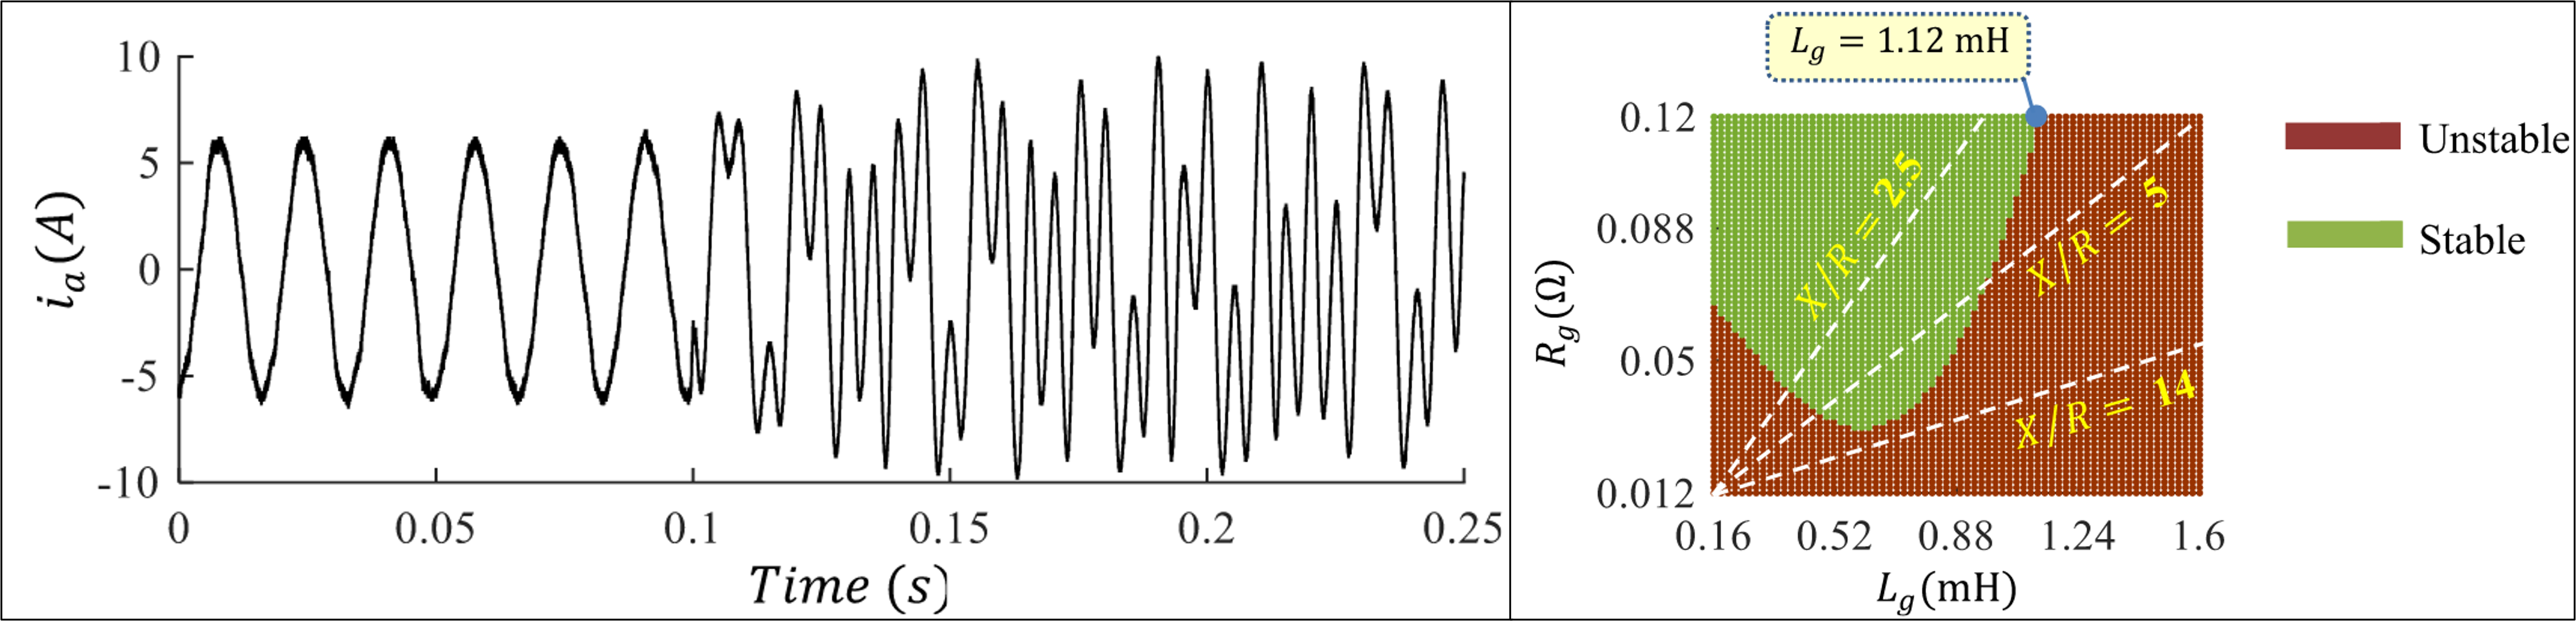
\includegraphics[scale=0.5]{stability_reg}
    }
    \caption{The stable and unstable regions with respect to X/R ratio \cite{8242351}.}\label{fig:stability_regions}
\end{figure}

The transition to PEDGs, driven by the integration of distributed generation, EVs and storage systems, introduces significant operational challenges evolving from low inertia, rapid dynamics, bidirectional power flow and stochastic behavior. The European project MIGRATE has outlined in \autocite{MIGRATE2016} the primary technical challenges associated with the extensive integration of IBRs into the grid. These challenges are summarized in Table \ref{tab:power_system_issues}, which was generalized for different level of systems and presented in Figure~\cref{fig:general_issues}  in \autocite{8809097}.

\begin{table} [htbp]
    \centering
    \begin{threeparttable}% выравнивание подписи по границам таблицы
        \caption{Ranked Issues in Power Systems}\label{tab:power_system_issues}%
        \begin{tabular}{| c || p{13cm} |}
            \hline
            \hline
                \textbf{Rank} & \textbf{Issue} \\ \hline
                1 & Decrease of inertia \\ \hline
                2 & Resonances due to cables and IBR \\ \hline
                3 & Reduction of transient stability margins \\ \hline
                4 & Missing or wrong participation of IBR-connected generators and loads in frequency containment \\ \hline
                5 & IBR Controller interaction with each other and passive AC components \\ \hline
                6 & Loss of devices in the context of fault-ride-through capability \\ \hline
                7 & Lack of reactive power \\ \hline
                8 & Introduction of new power oscillations and/or reduced damping of existing power oscillations \\ \hline
                9 & Excess of reactive power \\ \hline
                10 & Voltage dip-induced frequency dip \\ \hline
                11 & Altered static and dynamic voltage dependence of loads \\ \hline
            \hline
        \end{tabular}
    \end{threeparttable}
\end{table}

\begin{figure}[ht]
    \centerfloat{
        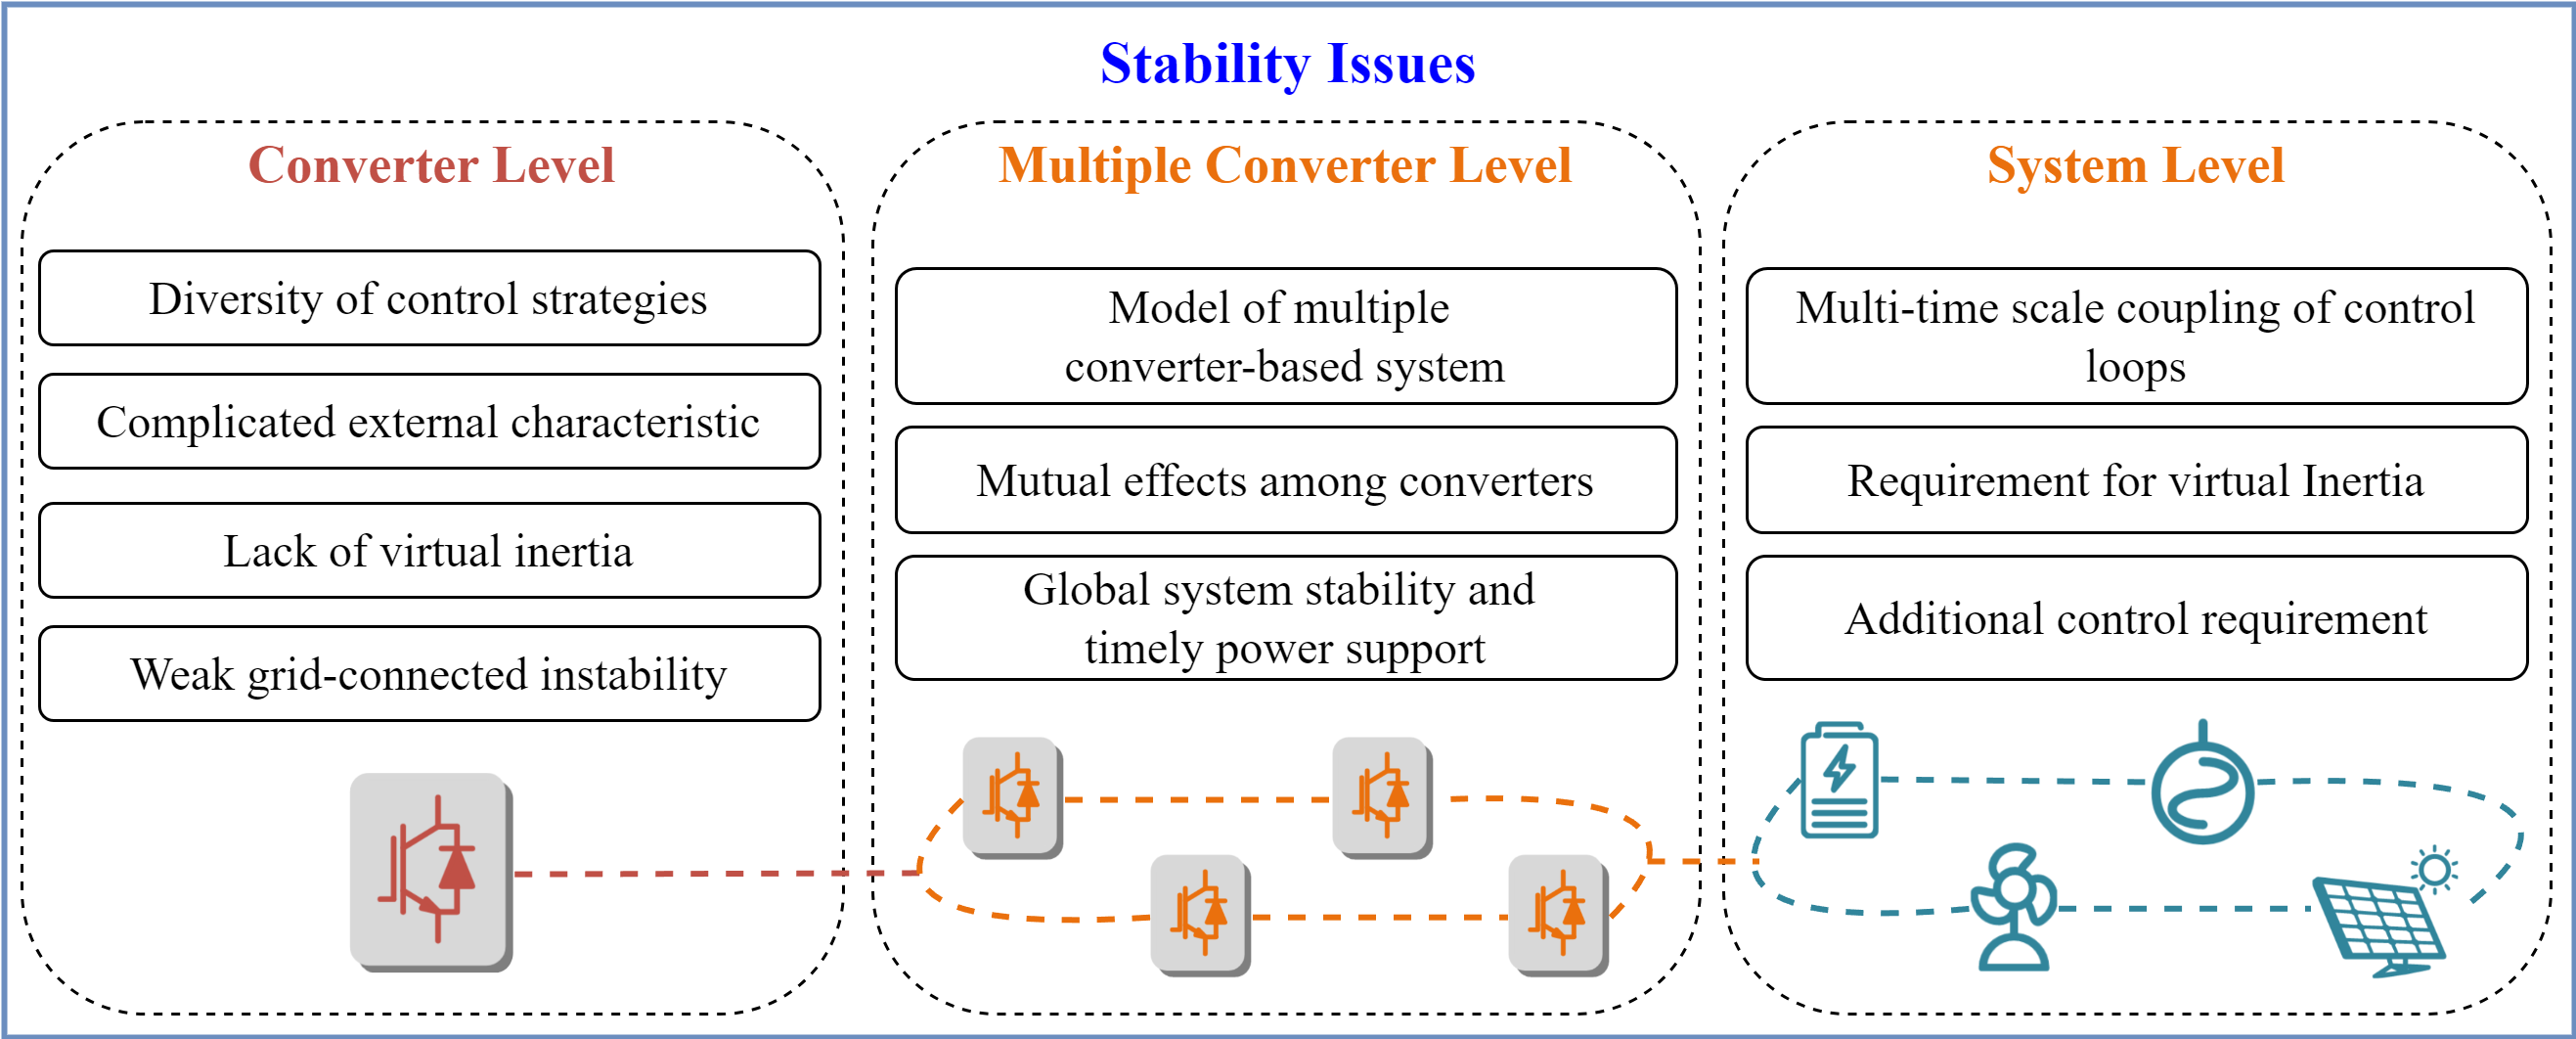
\includegraphics[scale=0.7]{general_issues}
    }
    \caption{General issues of PEDGs.}\label{fig:general_issues}
\end{figure}

Such characteristics require a paradigm shift in grid management, demanding real-time system awareness beyond the capabilities of traditional monitoring methods. The diverse timescales of PEDG dynamics, from microsecond-level converter control to minute-level demand-supply balancing, require fast and accurate dynamic state tracking to enable rapid instability detection, dynamic control and protection coordination, adaptive protection schemes, and optimized reactive power management. Maintaining secure operation of the system is one of the priority tasks, which critically depends on the system's overall observability.


\textbf{Moving Towards a DT-centric EMS Architecture.}
The electrical power system contains a transmission system, sub-transmission system, and distribution systems \autocite{kundur1994power}. As can be seen from Figure~\cref{fig:ps_illustration}, there is a comprehensive electrical interconnection among all components of the power system, whereas different voltage levels are interfaced by transformers. The fundamental role of a power system is to deliver electrical energy that meets predefined standards of quality, adequacy, reliability, and economic efficiency. 

\begin{figure}[ht]
    \centerfloat{
        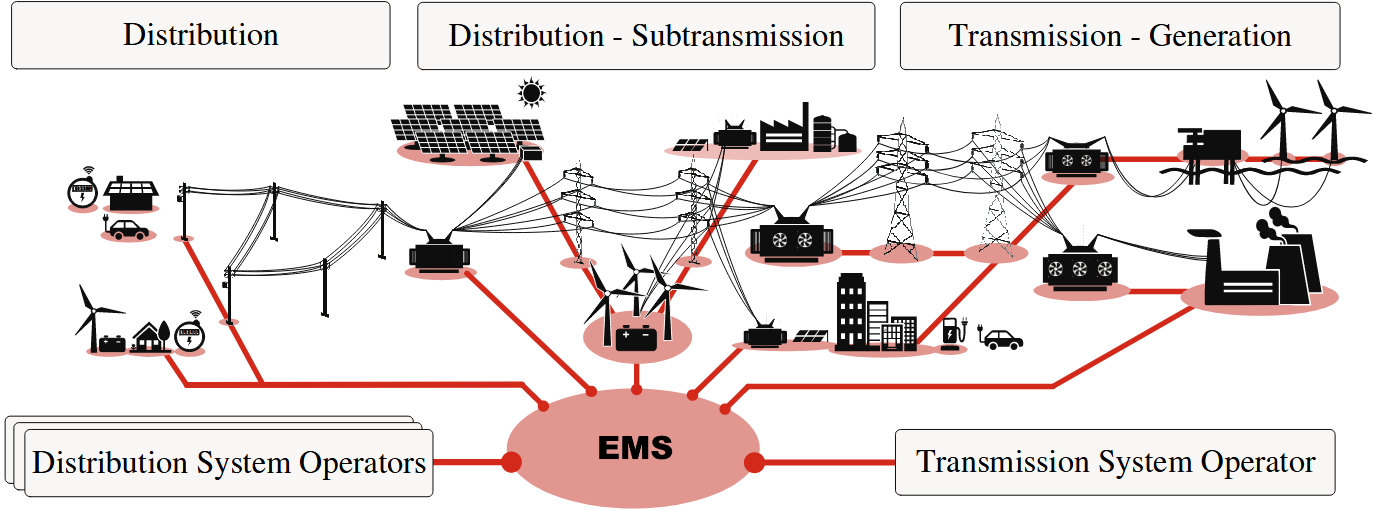
\includegraphics[scale=0.4]{ps_illustration_ems}
    }
    \caption{Illustration of modern power system \cite{Prostejovsky2017}.}\label{fig:ps_illustration}
\end{figure}

However, beyond these physical connections, maintaining secure operation critically depends on the system's overall observability. This real-time awareness of the operational state is accomplished through the deployment of numerous sensors, robust data processing infrastructure, and sophisticated information and communication technologies (ICT). The integration of the physical power infrastructure with this digital layer of monitoring and control establishes the modern power grid as a cyber-physical system. 

\nomenclature{\(ICT\)}{Information and Communication Technologies}

As the central "nerve system" of a cyber-physical entity, the Energy Management System (EMS) is designed to monitor, control, and optimize the generation, transmission, and distribution of electrical power. The aforementioned challenges in microgrid operation and control increase the complexity to EMS functioning as well. Among these intricacy's: 

\nomenclature{\(EMS\)}{Energy Management System}

\begin{itemize}
    \item Rapid change in power system operation challenges human operators in their supervision and control duties \autocite{cigre_700}.
    
    \item Complex dynamic phenomena of PEDG reduce reaction time and the capability of humans to react appropriately. This raises the risk of human errors subjected to time pressure \autocite{HAASS20155285}.
    
    \item Online dynamic security assessments (DSA) were traditionally used during planning and system design. Currently, annual dynamic stability assessments are required to determine stability limits \autocite{european_union_2017_1485}. The focus on dynamic system models has since advanced towards real-time operations.

    \item  Operating the system closer to its physical boundaries \autocite{8295027}, as necessitated by the energy transition, means that understanding and predicting these fast dynamic phenomena becomes crucial for maintaining operational security in EMS.
    
\end{itemize}

\nomenclature{\(DSA\)}{Dynamic Security Assessment}

Thus, as a response to EMS needs to address possible future scenarios and utility needs, the concept of the Digital Twin (DT) appears. Generally, DTs are digital replicas of systems, processes, or objects that mirror their physical state through abstraction and connect the physical and digital realms through sensor data streams \autocite{10311709}. The concept showed potential for applications that need improved observability and prediction of future conditions and system states. \autocite{eyre_untangling_2020}. Among the main characteristics, DT incorporates:
\begin{enumerate}
    \item A robust analytical model derived from the digital replica of the actual system \autocite{Trauer_2020},
    \item Real-time bidirectional data interaction \autocite{VANDERHORN2021113524},
    \item Accurate state reflection of the linked physical entity \autocite{JONES202036}.
\end{enumerate}

\nomenclature{\(DT\)}{Digital Twin}

Simply saying, a Digital Twin can be described dynamically updating model providing analytical insights into its mirrored system , distinguishing itself from traditional simulation models by ability to stay synchronous to the connected system. Table \ref{tab:ems_evol} illustrates the evolution of the power system evolving into a highly integrated cyber-physical system, with the DT concept as a key component of the EMS.

\begin{table} [htbp]
    \centering
    \begin{threeparttable}% выравнивание подписи по границам таблицы
        \caption{Evolution of EMS \autocite{8398846}}\label{tab:ems_evol}%
        \begin{tabular}{| c || p{5cm} | p{8cm} |}
            \hline
            \hline
                 \textbf{Generation} & \textbf{EMS Features} & \textbf{Functionality}\\ \hline
                1st & Analog communication via hardwired connections & Essential measurement values are displayed using a basic human-machine interface \\ \hline
                2nd & IP/TCP based  communication & SCADA and state estimation allow quasi steady-state observability \\ \hline
                3rd & Support of dynamic  observability & Wide area monitoring and dynamic security assessment tool available \\ \hline
                4th & Digital Twin centric architecture & Real-time simulation of high-fidelity models is a core functionality \\ \hline
            \hline
        \end{tabular}
    \end{threeparttable}
\end{table}

From the third generation of EMS, with its dynamic power system observability, the next advance is expected to be towards a DT-centric EMS architecture \autocite{dbt_mods_00054812}. In the core of that system, a modeling engine, a so-called \textit{dynamic digital mirror} (DDM), which supports real-time dynamic power system simulations. The primary focus of this research is on developing \textit{dynamic mirroring} specifically tailored for PEDGs.

\nomenclature{\(DDM\)}{Dynamic Digital Mirror}

The time-domain simulation engine, linked to the validated DT simulation model, allows precise state representation of the observed power system. This dynamic digital mirror engine aids in accurately estimating the power system state and provides a validated model foundation, potentially facilitating online power system studies like dynamic security analysis, state health monitoring, forecasting, event identification, relay protection and cyber security. The proposed method is evaluated through case studies using real-time numerical time-domain simulations, aiming for accurate and reliable dynamic mirroring.

{\aim} of the study is to develop a method for dynamic mirroring in PEDGs using a digital twin approach. 

To achieve the goal of the dissertation, the following {\tasks} are addressed:
\begin{enumerate}[beginpenalty=10000] % https://tex.stackexchange.com/a/476052/104425
  \item To propose an architecture of digital dynamic mirroring for the next generation of monitoring system.
  \item To develop an accurate and computationally effective modeling approach for a power system DT.
  \item To develop DT simulation engine to run real-time dynamic PEDG simulations.
  \item To develop of corresponding communication interfaces to apply the dynamic mirroring for online system monitoring.
\end{enumerate}


{\novelty} which are also {\defpositions}
\begin{enumerate}[beginpenalty=10000] % https://tex.stackexchange.com/a/476052/104425
  \item Validated dynamic average models for key components suitable for representation of dynamics of PEDG in real-time simulation.
  \item A novel DT framework for dynamic mirroring in PEDGs.
  \item Analysis of the sensitivity of the DT-based DDM to parameter deviations and data latency.
\end{enumerate}

{\influence} of the research. The main conclusions of the dissertation research can be used for developing the core component of next-generation DT-centric EMS, a suitable modeling engine, which allows for mirroring the actual power system state to support control, decision-making, and to execute simulations to predict future states. 

% The thesis presents the novel approach for DDM as a part of the next generation EMS. The effective modeling approach and simulation engine for real-time DT model execution developed by author.

{\methods} The methodology is based on applying discrete time state-space modeling for real-time simulation engine to run the dynamic model of PEDG. The research is based on comprehensive analysis of fast dynamics which appear in PEDG and arise from the interaction of numerous IBRs and transmission lines. The research include inverter grid-following mode dynamic modeling on behalf of TL and loads.  The research was validated through numerical real-time simulations and laboratory experiments based on hardware-in-the-loop approach. 

% {\defpositions}
% \begin{enumerate}[beginpenalty=10000] % https://tex.stackexchange.com/a/476052/104425
%   \item Первое положение
%   \item Второе положение
%   \item Третье положение
%   \item Четвертое положение
% \end{enumerate}
% В папке Documents можно ознакомиться с решением совета из Томского~ГУ
% (в~файле \verb+Def_positions.pdf+), где обоснованно даются рекомендации
% по~формулировкам защищаемых положений.


{\reliability} were confirmed by numerical simulation and experimental validation with hardware-in-loop approach involved de facto RTDS and OPAL-RT tools for the closed-loop testing of electrical hardware systems. The statements and conclusions formulated in the dissertation have been approved by the committees of experts in international scientific conferences. The credibility is also confirmed by the publications of research results in peer-reviewed scientific journals. 


{\probation}
The results of the dissertation were presented at the following international conferences:
\begin{itemize}
    \item 25th International Conference of Young Professionals in Electron Devices and Materials (2024 EDM).
    \item Conference of Young Researchers in Electrical and Electronic Engineering (2025 ElCon)
\end{itemize}

{\contribution} The personal contribution of the author includes proposing the idea of dynamic mirroring based on DT approach. To prove it, the author develop computationally efficient dynamic average models of PEDG for real-time execution, aiming to provide accurate and timely grid observability, even during transient events. For testing, hardware-in-the-loop test bench was developed, including physical grid representation and a DT model with data measurement interaction between them. All real-time simulations were performed and finally validated through experiments. 

% \ifnumequal{\value{bibliosel}}{0}
% {%%% Встроенная реализация с загрузкой файла через движок bibtex8. (При желании, внутри можно использовать обычные ссылки, наподобие `\cite{vakbib1,vakbib2}`).
%     {\publications} Основные результаты по теме диссертации изложены
%     в~XX~печатных изданиях,
%     X из которых изданы в журналах, рекомендованных ВАК,
%     X "--- в тезисах докладов.
% }%
% {%%% Реализация пакетом biblatex через движок biber
%     \begin{refsection}[bl-author, bl-registered]
%         % Это refsection=1.
%         % Процитированные здесь работы:
%         %  * подсчитываются, для автоматического составления фразы "Основные результаты ..."
%         %  * попадают в авторскую библиографию, при usefootcite==0 и стиле `\insertbiblioauthor` или `\insertbiblioauthorgrouped`
%         %  * нумеруются там в зависимости от порядка команд `\printbibliography` в этом разделе.
%         %  * при использовании `\insertbiblioauthorgrouped`, порядок команд `\printbibliography` в нём должен быть тем же (см. biblio/biblatex.tex)
%         %
%         % Невидимый библиографический список для подсчёта количества публикаций:
%         \phantom{\printbibliography[heading=nobibheading, section=1, env=countauthorvak,          keyword=biblioauthorvak]%
%         \printbibliography[heading=nobibheading, section=1, env=countauthorwos,          keyword=biblioauthorwos]%
%         \printbibliography[heading=nobibheading, section=1, env=countauthorscopus,       keyword=biblioauthorscopus]%
%         \printbibliography[heading=nobibheading, section=1, env=countauthorconf,         keyword=biblioauthorconf]%
%         \printbibliography[heading=nobibheading, section=1, env=countauthorother,        keyword=biblioauthorother]%
%         \printbibliography[heading=nobibheading, section=1, env=countregistered,         keyword=biblioregistered]%
%         \printbibliography[heading=nobibheading, section=1, env=countauthorpatent,       keyword=biblioauthorpatent]%
%         \printbibliography[heading=nobibheading, section=1, env=countauthorprogram,      keyword=biblioauthorprogram]%
%         \printbibliography[heading=nobibheading, section=1, env=countauthor,             keyword=biblioauthor]%
%         \printbibliography[heading=nobibheading, section=1, env=countauthorvakscopuswos, filter=vakscopuswos]%
%         \printbibliography[heading=nobibheading, section=1, env=countauthorscopuswos,    filter=scopuswos]}%
%         %
%         \nocite{*}%
%         %
%         {\publications} Основные результаты по теме диссертации изложены в~\arabic{citeauthor}~печатных изданиях,
%         \arabic{citeauthorvak} из которых изданы в журналах, рекомендованных ВАК%
%         \ifnum \value{citeauthorscopuswos}>0%
%             , \arabic{citeauthorscopuswos} "--- в~периодических научных журналах, индексируемых Web of~Science и Scopus%
%         \fi%
%         \ifnum \value{citeauthorconf}>0%
%             , \arabic{citeauthorconf} "--- в~тезисах докладов.
%         \else%
%             .
%         \fi%
%         \ifnum \value{citeregistered}=1%
%             \ifnum \value{citeauthorpatent}=1%
%                 Зарегистрирован \arabic{citeauthorpatent} патент.
%             \fi%
%             \ifnum \value{citeauthorprogram}=1%
%                 Зарегистрирована \arabic{citeauthorprogram} программа для ЭВМ.
%             \fi%
%         \fi%
%         \ifnum \value{citeregistered}>1%
%             Зарегистрированы\ %
%             \ifnum \value{citeauthorpatent}>0%
%             \formbytotal{citeauthorpatent}{патент}{}{а}{}%
%             \ifnum \value{citeauthorprogram}=0 . \else \ и~\fi%
%             \fi%
%             \ifnum \value{citeauthorprogram}>0%
%             \formbytotal{citeauthorprogram}{программ}{а}{ы}{} для ЭВМ.
%             \fi%
%         \fi%
%         % К публикациям, в которых излагаются основные научные результаты диссертации на соискание учёной
%         % степени, в рецензируемых изданиях приравниваются патенты на изобретения, патенты (свидетельства) на
%         % полезную модель, патенты на промышленный образец, патенты на селекционные достижения, свидетельства
%         % на программу для электронных вычислительных машин, базу данных, топологию интегральных микросхем,
%         % зарегистрированные в установленном порядке.(в ред. Постановления Правительства РФ от 21.04.2016 N 335)
%     \end{refsection}%
%     \begin{refsection}[bl-author, bl-registered]
%         % Это refsection=2.
%         % Процитированные здесь работы:
%         %  * попадают в авторскую библиографию, при usefootcite==0 и стиле `\insertbiblioauthorimportant`.
%         %  * ни на что не влияют в противном случае
%         \nocite{vakbib2}%vak
%         \nocite{patbib1}%patent
%         \nocite{progbib1}%program
%         \nocite{bib1}%other
%         \nocite{confbib1}%conf
%     \end{refsection}%
%         %
%         % Всё, что вне этих двух refsection, это refsection=0,
%         %  * для диссертации - это нормальные ссылки, попадающие в обычную библиографию
%         %  * для автореферата:
%         %     * при usefootcite==0, ссылка корректно сработает только для источника из `external.bib`. Для своих работ --- напечатает "[0]" (и даже Warning не вылезет).
%         %     * при usefootcite==1, ссылка сработает нормально. В авторской библиографии будут только процитированные в refsection=0 работы.
% }

% При использовании пакета \verb!biblatex! будут подсчитаны все работы, добавленные
% в файл \verb!biblio/author.bib!. Для правильного подсчёта работ в~различных
% системах цитирования требуется использовать поля:
% \begin{itemize}
%         \item \texttt{authorvak} если публикация индексирована ВАК,
%         \item \texttt{authorscopus} если публикация индексирована Scopus,
%         \item \texttt{authorwos} если публикация индексирована Web of Science,
%         \item \texttt{authorconf} для докладов конференций,
%         \item \texttt{authorpatent} для патентов,
%         \item \texttt{authorprogram} для зарегистрированных программ для ЭВМ,
%         \item \texttt{authorother} для других публикаций.
% \end{itemize}
% Для подсчёта используются счётчики:
% \begin{itemize}
%         \item \texttt{citeauthorvak} для работ, индексируемых ВАК,
%         \item \texttt{citeauthorscopus} для работ, индексируемых Scopus,
%         \item \texttt{citeauthorwos} для работ, индексируемых Web of Science,
%         \item \texttt{citeauthorvakscopuswos} для работ, индексируемых одной из трёх баз,
%         \item \texttt{citeauthorscopuswos} для работ, индексируемых Scopus или Web of~Science,
%         \item \texttt{citeauthorconf} для докладов на конференциях,
%         \item \texttt{citeauthorother} для остальных работ,
%         \item \texttt{citeauthorpatent} для патентов,
%         \item \texttt{citeauthorprogram} для зарегистрированных программ для ЭВМ,
%         \item \texttt{citeauthor} для суммарного количества работ.
% \end{itemize}
% % Счётчик \texttt{citeexternal} используется для подсчёта процитированных публикаций;
% % \texttt{citeregistered} "--- для подсчёта суммарного количества патентов и программ для ЭВМ.

% Для добавления в список публикаций автора работ, которые не были процитированы в
% автореферате, требуется их~перечислить с использованием команды \verb!\nocite! в
% \verb!Synopsis/content.tex!.
 % Характеристика работы по структуре во введении и в автореферате не отличается (ГОСТ Р 7.0.11, пункты 5.3.1 и 9.2.1), потому её загружаем из одного и того же внешнего файла, предварительно задав форму выделения некоторым параметрам

\textbf{Объем и структура работы.} Диссертация состоит из~введения,
\formbytotal{totalchapter}{глав}{ы}{}{},
заключения и
\formbytotal{totalappendix}{приложен}{ия}{ий}{}.
%% на случай ошибок оставляю исходный кусок на месте, закомментированным
%Полный объём диссертации составляет  \ref*{TotPages}~страницу
%с~\totalfigures{}~рисунками и~\totaltables{}~таблицами. Список литературы
%содержит \total{citenum}~наименований.
%
Полный объём диссертации составляет
\formbytotal{TotPages}{страниц}{у}{ы}{}, включая
\formbytotal{totalcount@figure}{рисун}{ок}{ка}{ков} и
\formbytotal{totalcount@table}{таблиц}{у}{ы}{}.
Список литературы содержит
\formbytotal{citenum}{наименован}{ие}{ия}{ий}.
